\section{Methodology}

\begin{figure}[t]
\centering
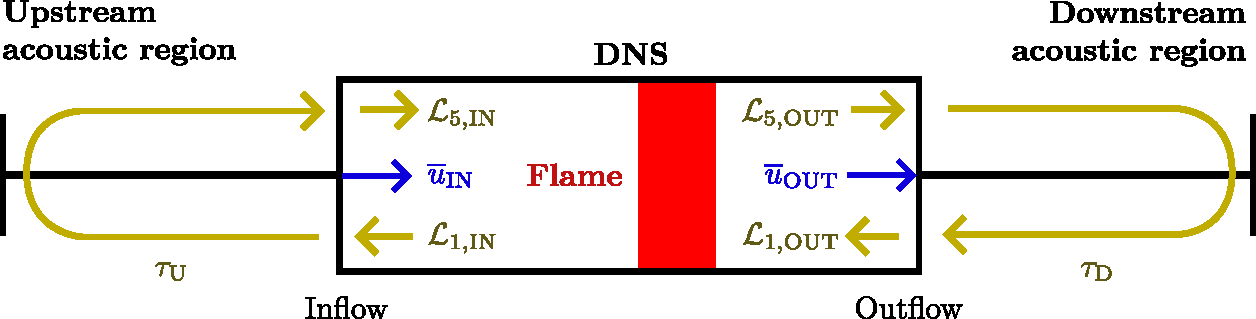
\includegraphics[scale=0.65]{assets/imgs/delay_bc_model.pdf}
\label{fig:delay-model}
\caption{MODEL OF DELAY BC. DELAY IS ONLY MODELLED VIA TIME SERIES OF L VALUES AS THEY LEAVE THE DNS DOMAIN.}
\end{figure}


% Outline the idea
% How does this connect to the NSCBC formalism
% Remove P controllers/relaxation terms
% Leave in diffusion boundaries to get a well-posed problem
% Memory footprint



\section{Implementation}


\subsection{Code Schematic}

\begin{figure}[t]
\centering
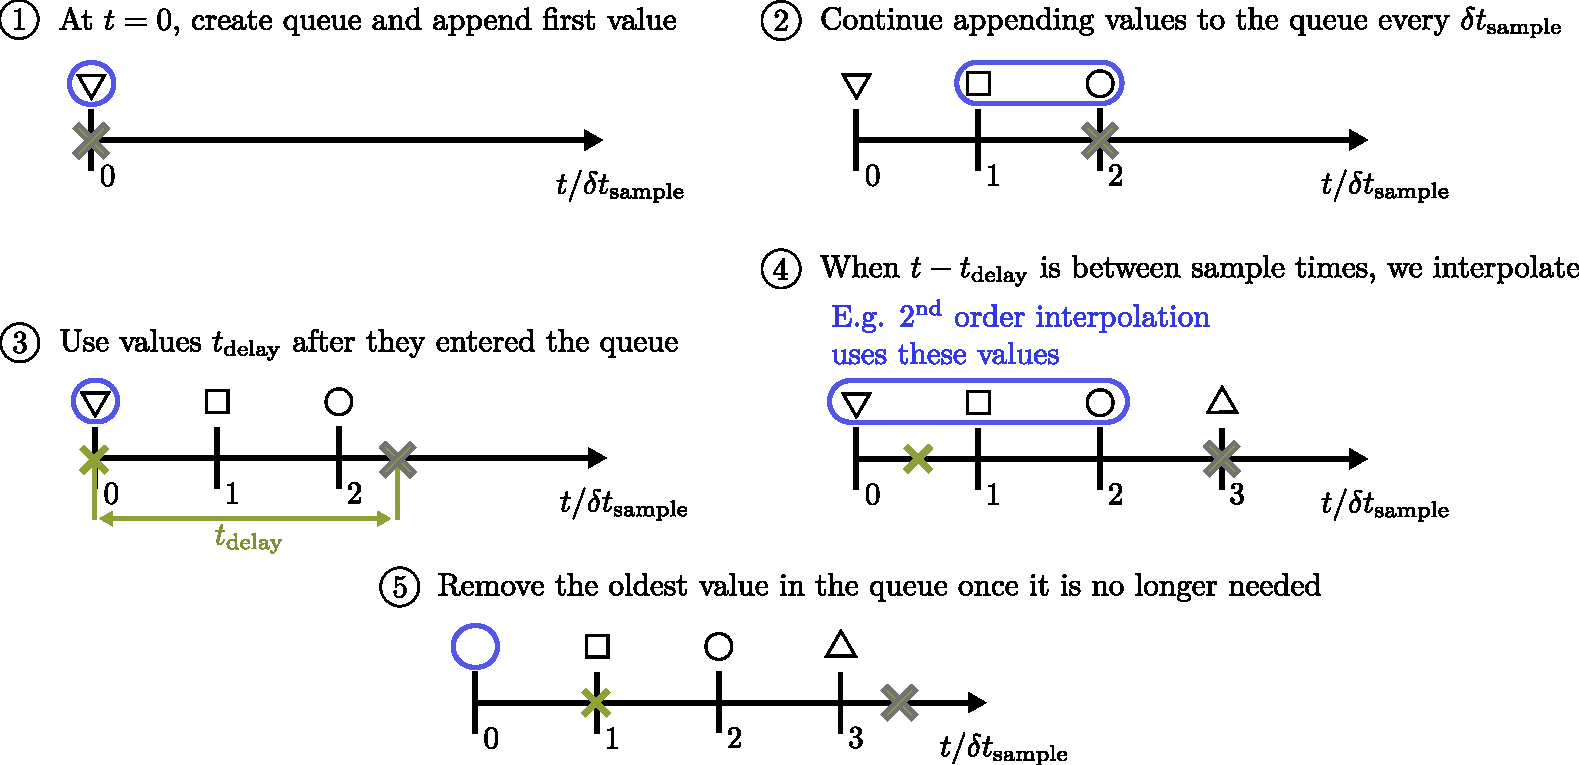
\includegraphics[scale=0.65]{assets/imgs/delay_bc_queue.pdf}
\label{fig:delay-queue}
\caption{HOW THE BOUNDARY SAMPLING AND DELAY WORK. WHAT DO SHAPES REPRESENT?? GREY CROSS IS CURRENT SIMULATION TIME, GOLD CROSS IS THAT TIME MINUS THE TIME DELAY. CHANGING TIME DELAY IS NOT SHOWN HERE.}
\end{figure}

\begin{figure}[t]
\centering
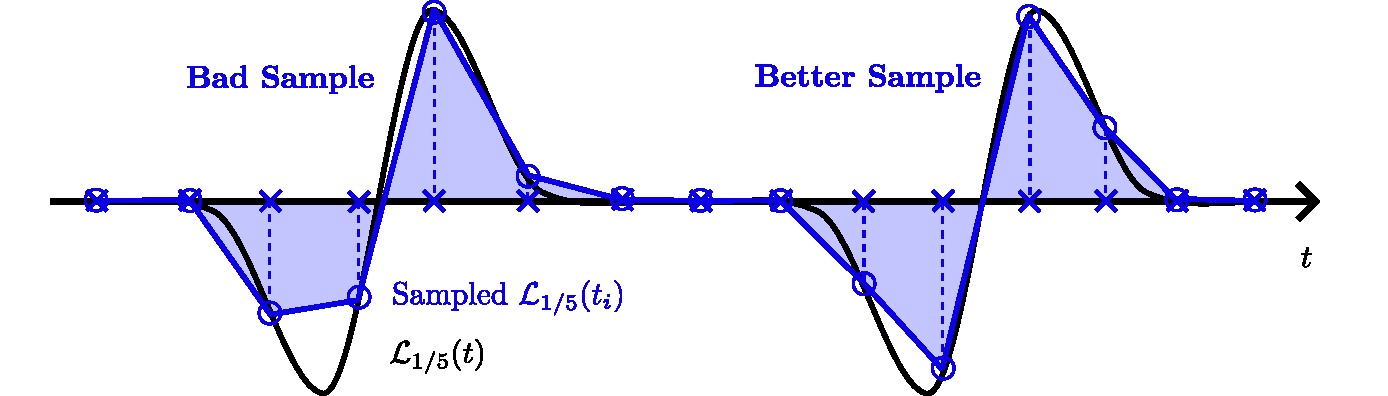
\includegraphics[scale=0.65]{assets/imgs/wave-sampling-comparison.pdf}
\caption{SAMPLING}
\label{fig:wave-sampling}
\end{figure}

% Now is a good time to bring up the sampling error
% - \fig{fig:wave-sampling} shows a representative analytic L_{1/5} field for two acoustic bumps (which is roughly the derivative of the Gaussian). Despite the same linear interpolation and sample period being used, the sampled $L$ values on the left are much worse than on the right. The same could be true for any number of samples at a constant interpolation order and sample period, where the change in phase of the sampling with the wave will always cause some inaccuracy in the integrated acoustic field. This inaccuracy results in a change to the shape of the Gaussian, e.g. a skew to one side, which feeds back into this issue such that the waves eventually fully break down
% - For the acoustic bump in this small domain this seems to happen relatively quickly because the associated acoustic frequencies of this system are higher. But, if the bump remains the same size and the tube is made longer, less bounces happen and the sampling error grows slower
% - Furthermore, there is the added effect that natural wavenumbers of these longer tubes will be lower, meaning that individual waves can be sampled better. This leads to an asymptotic behaviour of O(l^2) for values of error productions which are small (DO SOME MATHS?).




% CHANGE ITALIC L TO CALLIGRAPHIC L
\begin{figure}[t]
\centering
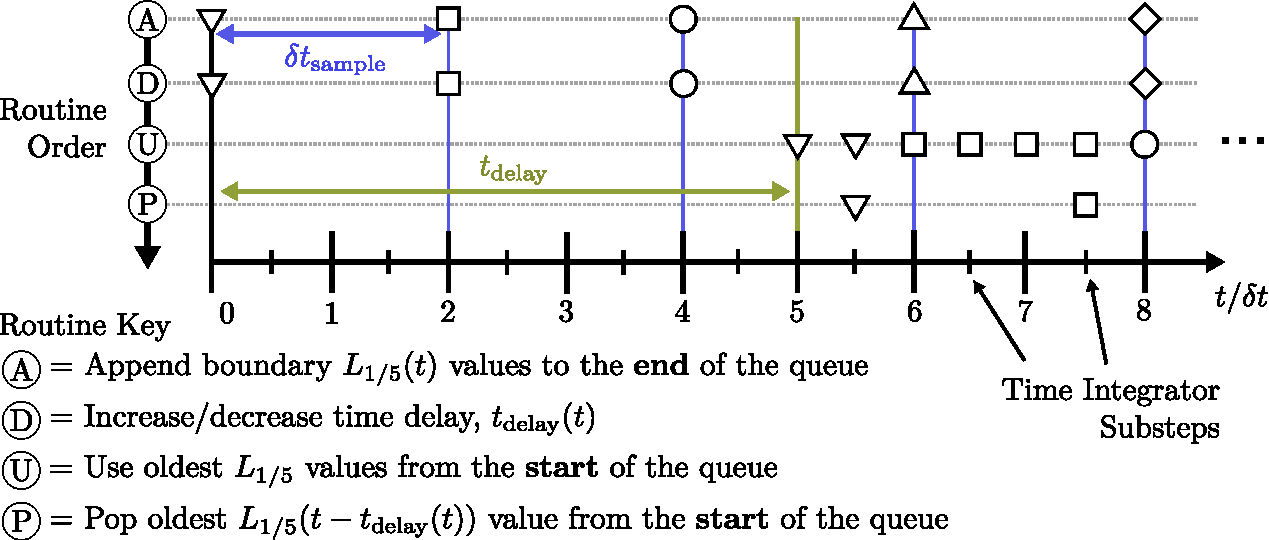
\includegraphics[scale=0.65]{assets/imgs/delay_bc_code_schematic.pdf}
\label{fig:schematic}
\caption{Schematic for delay BCs implemented into a multistage time integrator. ASSUMES CONSTANT TIME STEPS. TOP TO BOTTOM, LEFT TO RIGHT. BLUE SHOWS SAMPLE TIMES, GOLD SHOWS TIME DELAY}
\end{figure}


\begin{itemize}
\item Queues are filled with $L$ values as well as 
\end{itemize}



\subsection{Visualisation In The Acoustic Region}
% Maybe put into results if it makes more sense


% Acoustic region postprocessing
% - theoretically how could this work in the ADCBC framework?
% - log stored queue values at specific non-dimensional times which are interpreted as time series of characteristic waves leaving the inflow or outflow DNS boundary
% - According to the same linear approximation made on acoustic waves under the ADCBC formulation, we can reinterpret these time series as spatial information: the longer ago the acoustic exited the domain, the farther into the acoustic domain (or back towards the DNS domain) they will be
% - This only requires the queue information, sound speed and u to calculate upstream and downstream L_1 and L_5 values, then to calculate upstream and downstream u and p values we integrate L_1 and L_5 starting from the DNS inflow or outflow u and p alongside rho (for u?)





\subsection{Comparison with D-TDIBC}





